\documentclass[fleqn,10pt]{wlscirep}

%% define a new envrionment which marries longtable with tabulary
% from http://tex.stackexchange.com/questions/78075/multi-page-with-tabulary (see there for usage)
% with modifications taken from the ltxtable package to make captions work
\makeatletter

\def\ltabulary{%
	\def\endfirsthead{\\}%
	\def\endhead{\\}%
	\def\endfoot{\\}%
	\def\endlastfoot{\\}%
	\def\tabulary{%
		\def\TY@final{%
			\def\endfirsthead{\LT@end@hd@ft\LT@firsthead}%
			\def\endhead{\LT@end@hd@ft\LT@head}%
			\def\endfoot{\LT@end@hd@ft\LT@foot}%
			\def\endlastfoot{\LT@end@hd@ft\LT@lastfoot}%
			\longtable}%
		\let\endTY@final\endlongtable
		\TY@tabular}%
	\dimen@\columnwidth
	\advance\dimen@-\LTleft
	\advance\dimen@-\LTright
	\tabulary\dimen@}

\def\endltabulary{\endtabulary}

\makeatother


% Packages
\usepackage{cleveref}
\usepackage{booktabs}
\usepackage{tabulary, booktabs, longtable, ltcaption, ltabptch}
%\usepackage[referable]{threeparttablex}
\usepackage{gensymb}

\title{Network analysis of the hominin origin of Herpes Simplex virus 2 from fossil data}
%\shorttitle{Hominin origin of HSV2}
\author[1,2]{Simon Underdown}
\author[3]{Krishna Kumar}
\author[4,5,*]{Charlotte Houldcroft}
\affil[1]{Human Origins and Palaeoenvironmental Research Group (HOPE), Department of Anthropology \& Geography, Oxford Brookes University, Oxford, OX3 0BP, UK.}
\affil[2]{Leverhulme Centre for Human Evolutionary Studies, University of Cambridge, Henry Wellcome Building, Fitzwilliam Street, Cambridge, CB2 1QH, UK.}
\affil[3]{Computational Geomechanics, Cambridge University Engineering Department, Trumpington Street, Cambridge, CB2 1PZ, UK.}
\affil[4]{Division of Biological Anthropology, Department of Archaeology \& Anthropology, University of Cambridge, Cambridge, CB2 3QG, UK.}
\affil[5]{McDonald Institute for Archaeological Research, University of Cambridge, Downing Street, Cambridge, CB2 3ER, UK.}

\affil[*]{ch504@cam.ac.uk}

\keywords{network analysis, virology, human evolution, epidemiology, archaelogy}

\begin{abstract}
Herpes simplex virus 2 is a human herpesvirus found worldwide that causes genital lesions and more rarely causes encephalitis. This pathogen is most common in Africa, and particularly in central and east Africa, an area of particular significance for the evolution of modern humans. Unlike HSV1, HSV2 has not simply co-speciated with humans from their last common ancestor with primates. HSV2 jumped the species barrier between 1.4 and 3 MYA, most likely through an intermediate but unknown hominin species. 

In this paper, we use probability-based network analysis to determine the probable path between intermediate hosts of HSV2, from chimpanzees to modern humans, using paleoenvironmental data on the distribution of African tropical rainforest over the last 3 million years and data on the age and distribution of fossil species of hominin present in Africa between 1.4 and 3 MYA. Our model identifies \textit{Homo rudolfensis} as the most likely intermediate host of HSV2
\end{abstract}


\addbibresource{references.bib}

\begin{document}

\flushbottom
\maketitle
%
\thispagestyle{empty}

\textbf{Keywords}
network analysis; human evolution; infectious disease; epidemiology; archaeology

\section*{Introduction}

Herpes simplex virus 2 (HSV2) is a sexually transmitted human pathogen that causes genital lesions and, rarely, encephalitis (eg \citep{Tang2003}), and is associated with increased risk of HIV acquisition~\citep{Freeman2006}. After primary infection, the virus adopts a life cycle of latency punctuated by periods of lytic replication when new hosts can be infected through genital contact. The virus is related to the human oral pathogen herpes simplex virus 1 (HSV1). Both HSV1 and HSV2 are alphaherpesviruses, which are found in many primates~\citep{Wertheim2014}.

HSV2 was originally thought to have co-speciated with humans when our lineage diverged from that of chimpanzees, but recent comparisons of the HSV1, HSV2 and chimpanzee herpesvirus~\cite{Tang2003} (ChHV1) genomes suggests that HSV2 is in fact more closely related to ChHV1 than HSV13. This analysis also found that HSV2 diverged from ChHV1 between 1.4 and 3 MYA, and the authors inferred that an intermediate hominin served as a host for HSV2 before it introgressed into the ancestors of modern humans.

We argue that by combining fossil data on when and where different hominin species were likely to be present in Africa, the geographical range of modern chimpanzees and bonobos, and the reconstructed distribution of tropical rainforest habitat as a proxy for the past range of the chimp/bonobo ancestor, it will be possible to develop a model to statistically infer the species that facilitated the introgression of HSV2 in the modern human lineage defined here as beginning with \textit{Homo erectus}~\cite{Anton2016}. The ancestor-descendant relationship between \textit{Homo erectus} at c. 2.0 MYA and \textit{Homo sapiens} c. 200 KYA is an evolutionarily secure route of transmission for HSV2 to leave Africa as a modern human-borne virus. This produces a window of infection time that closes with the dispersal of \textit{Homo sapiens} out of Africa no later than 100 KYA~\cite{MirazonLahr2016}

\section*{Results}

The A* optimal graph traversal algorithm was used to evaluate the most probable intermediary host(s) of HSV2 between the ancestors of modern chimpanzees and bonobos (ancestral-chimpanzees or anc-chimps) and the ancestors of modern humans. Directed Acyclic Graphs (DAGs) linking potential HSV2 transmission hominins were developed, with edges representing the possible direction of transmission between different hominins. Two mathematical models: the Infection Prevalence (HSV2-IP) model and the Infection Transmission (HSV2-IT) model, were developed for estimating the probability of HSV2 infection/transmission between species based on their geo-spatial and temporal distributions and their proximity to rainforest. These probability models were used to populate the DAG edge costs and node heuristics. Bayesian network inference of the DAG was also used to determine the most probable intermediary hosts. Both the A* algorithm~\cref{fig:dag-ip,fig:dag-it} and the Bayesian network inference identified \textit{Homo rudolfensis} as the most probable intermediary host that transmitted HSV2 from ancestral-chimpanzees to the ancestors of modern humans. \Cref{table:hsv2} shows the probable HSV2 intermediary routes and their rankings based on the infection transmission models and Bayesian network inference.

\begin{table}
\caption{Probable intermediary hosts for HSV2 transmission}
\centering
\renewcommand{\arraystretch}{1.5}
\label{table:hsv2}
\begin{tabulary}{\linewidth}{LCCC}
\toprule
Disease Transmission Route & 
HSV2-IP route ranking
(normalised path cost) & 
HSV2-IT route ranking
(normalised path cost) & 
Bayesian inference (probability)
 \\ 
\midrule
anc-chimp $\Rightarrow$ \textit{rudolfensis} $\Rightarrow$ \textit{erectus} & \textbf{1 (0.0 \%)} & \textbf{1 (0.0 \%)} & \textbf{11.59\%} \\

anc-chimp $\Rightarrow$ \textit{boisei} $\Rightarrow$ \textit{erectus} & 2 (6.24 \%) & 4 (4.03 \%) & 9.28\% \\

anc-chimp $\Rightarrow$ \textit{habilis}  $\Rightarrow$ \textit{boisei} $\Rightarrow$ \textit{erectus} & 3 (7.97 \%) & 2 (1.92 \%) & 5\% \\

anc-chimp $\Rightarrow$ \textit{habilis} $\Rightarrow$ \textit{erectus} & 4 (10.91 \%) & 3 (3.39 \%) & 7.8\% \\
\bottomrule
\multicolumn{4}{l}{* \% path cost represents the normalised value with respect to the most and the least probable route.}\\
\multicolumn{4}{l}{The most probable route has a 0\% cost, and least probable route has an 100\% cost.}
\end{tabulary}
\end{table}

\begin{figure}
  \centering
  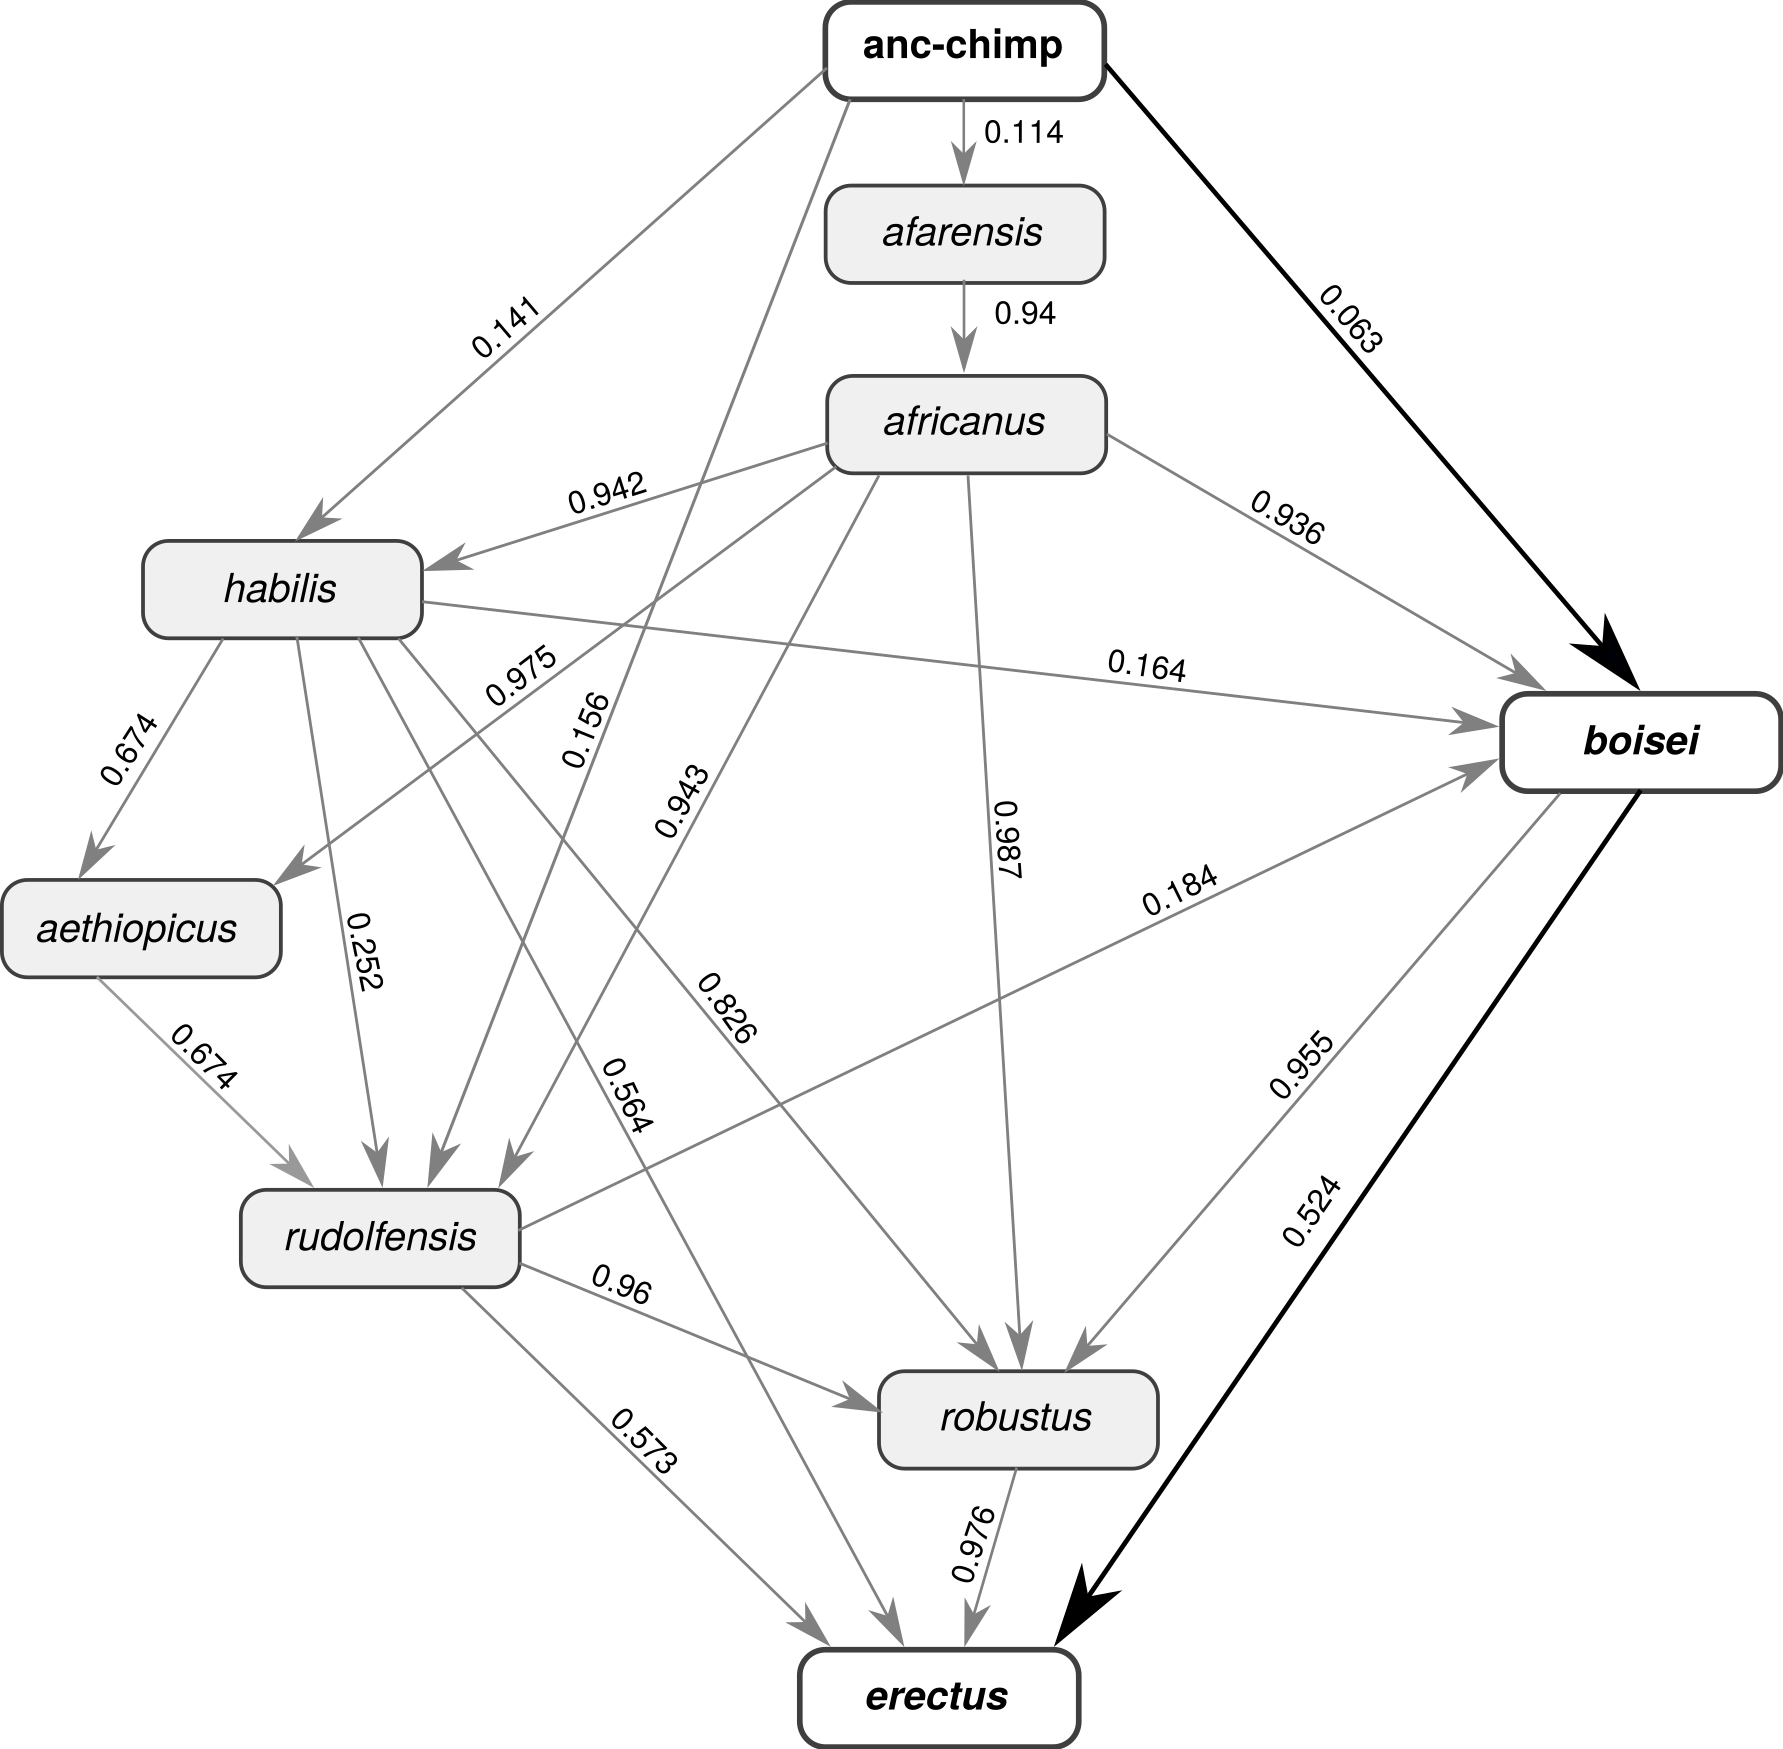
\includegraphics[width=\textwidth]{figs/dag-ip}
  \caption{A* shortest path for HSV2 Infection Prevalence (HSV2-IP) model}
  \label{fig:dag-ip}   
\end{figure}  

\begin{figure}
  \centering
  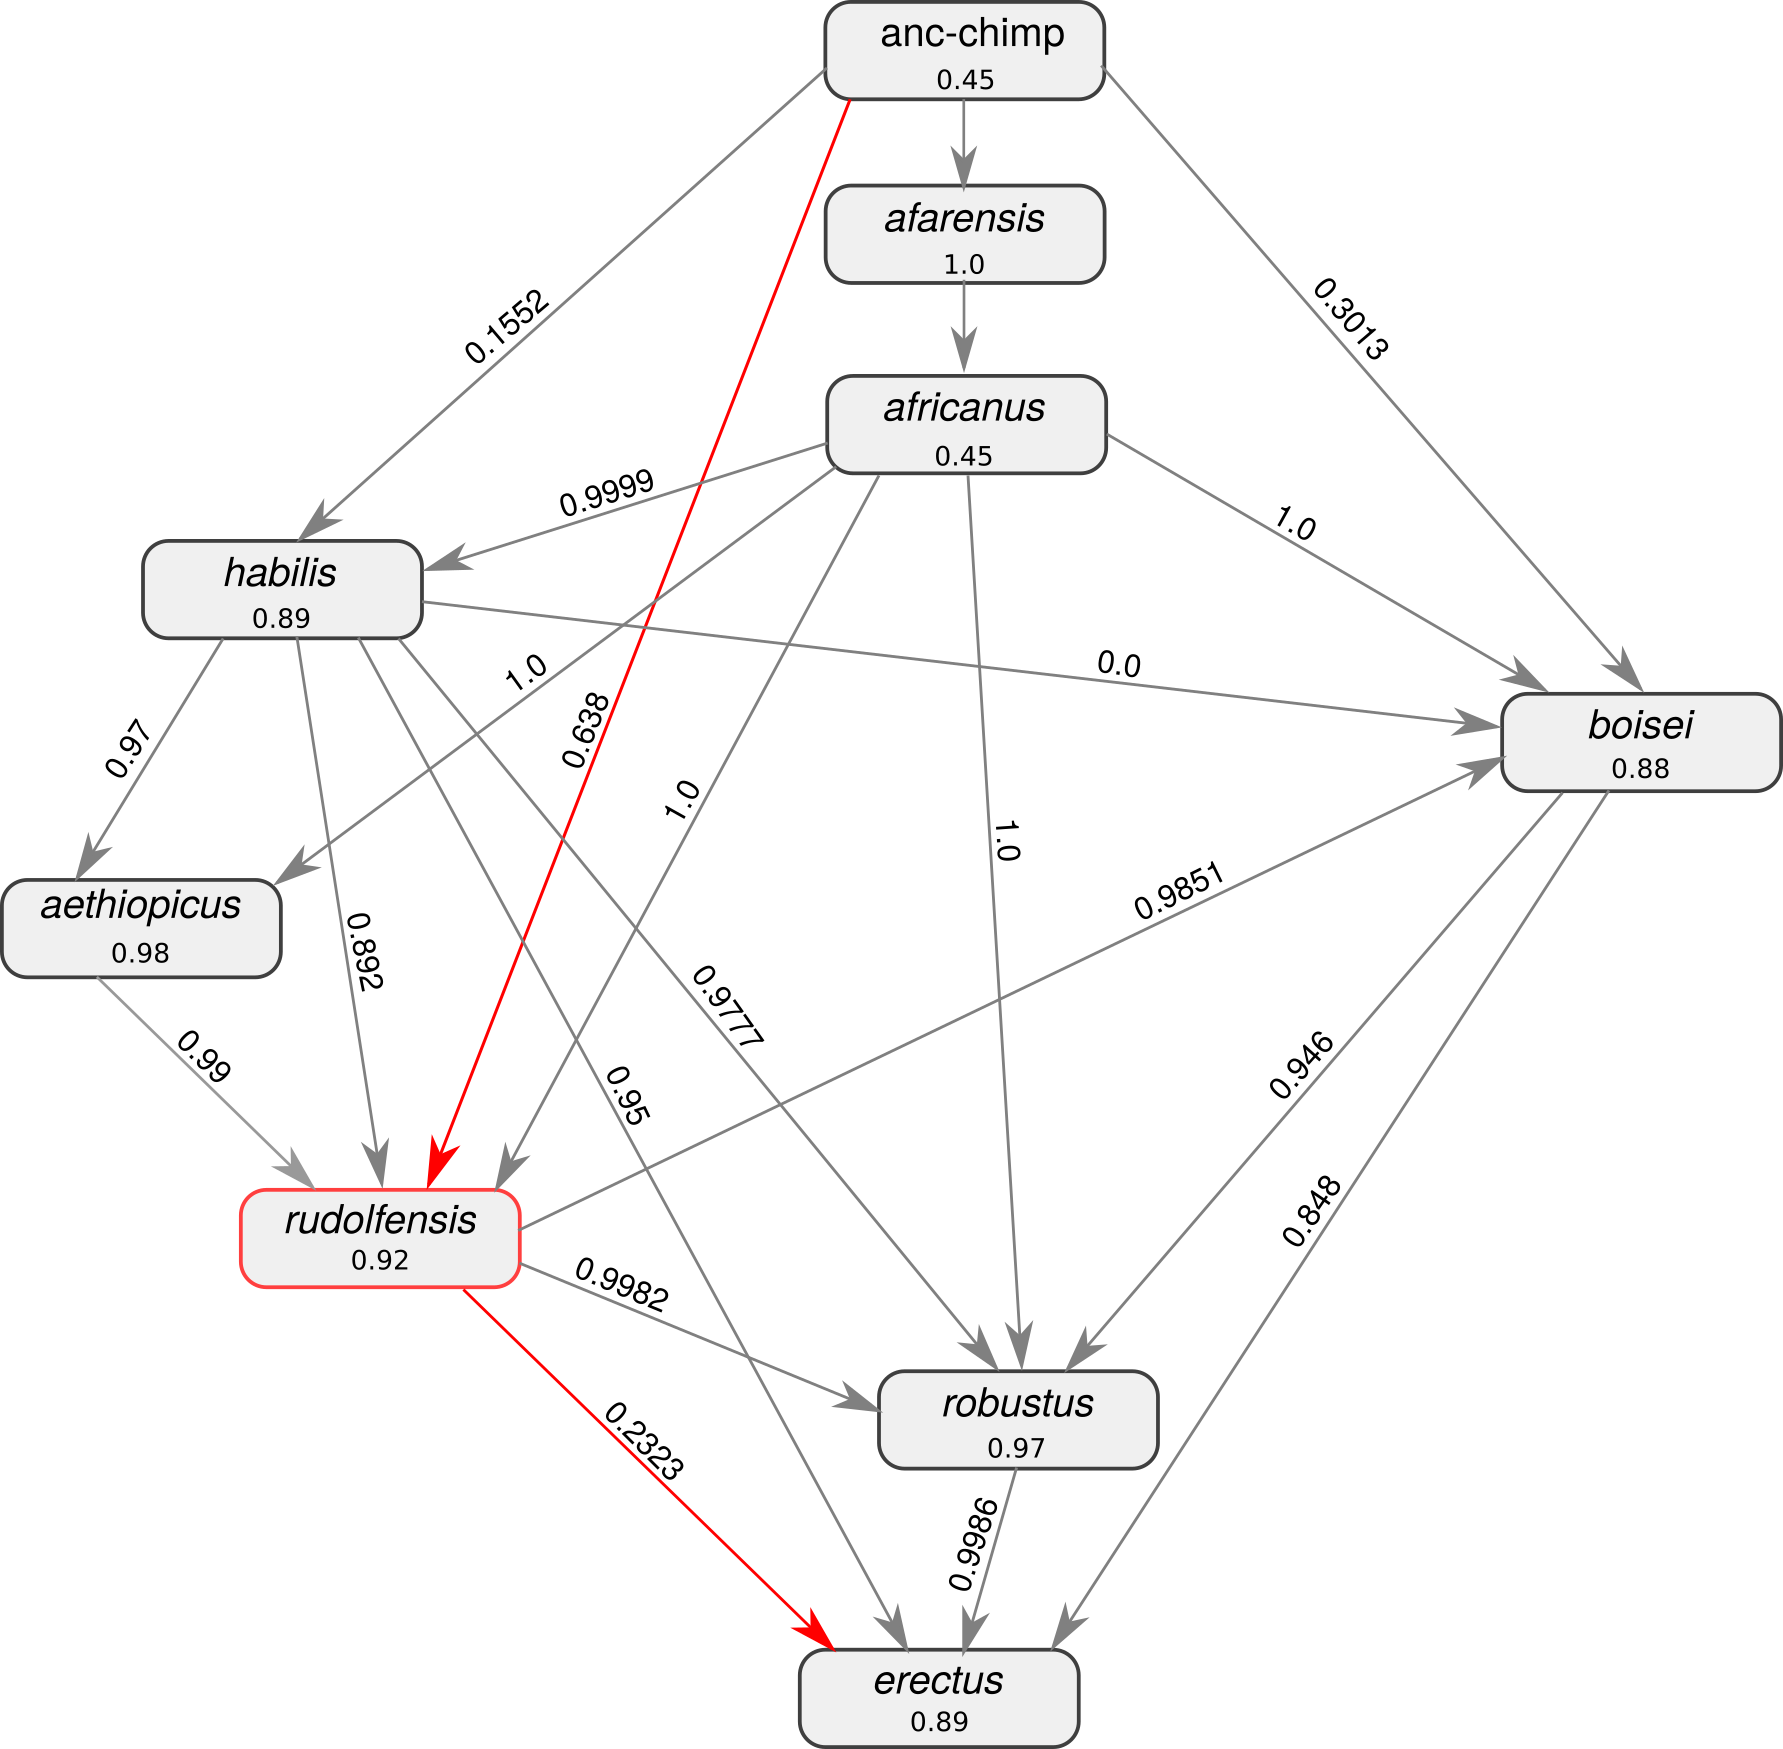
\includegraphics[width=\textwidth]{figs/dag-it}
  \caption{A* shortest path for HSV2 Infection Transmission (HSV2-IT) model}
  \label{fig:dag-it}   
\end{figure}     

\begin{figure}
  \centering
  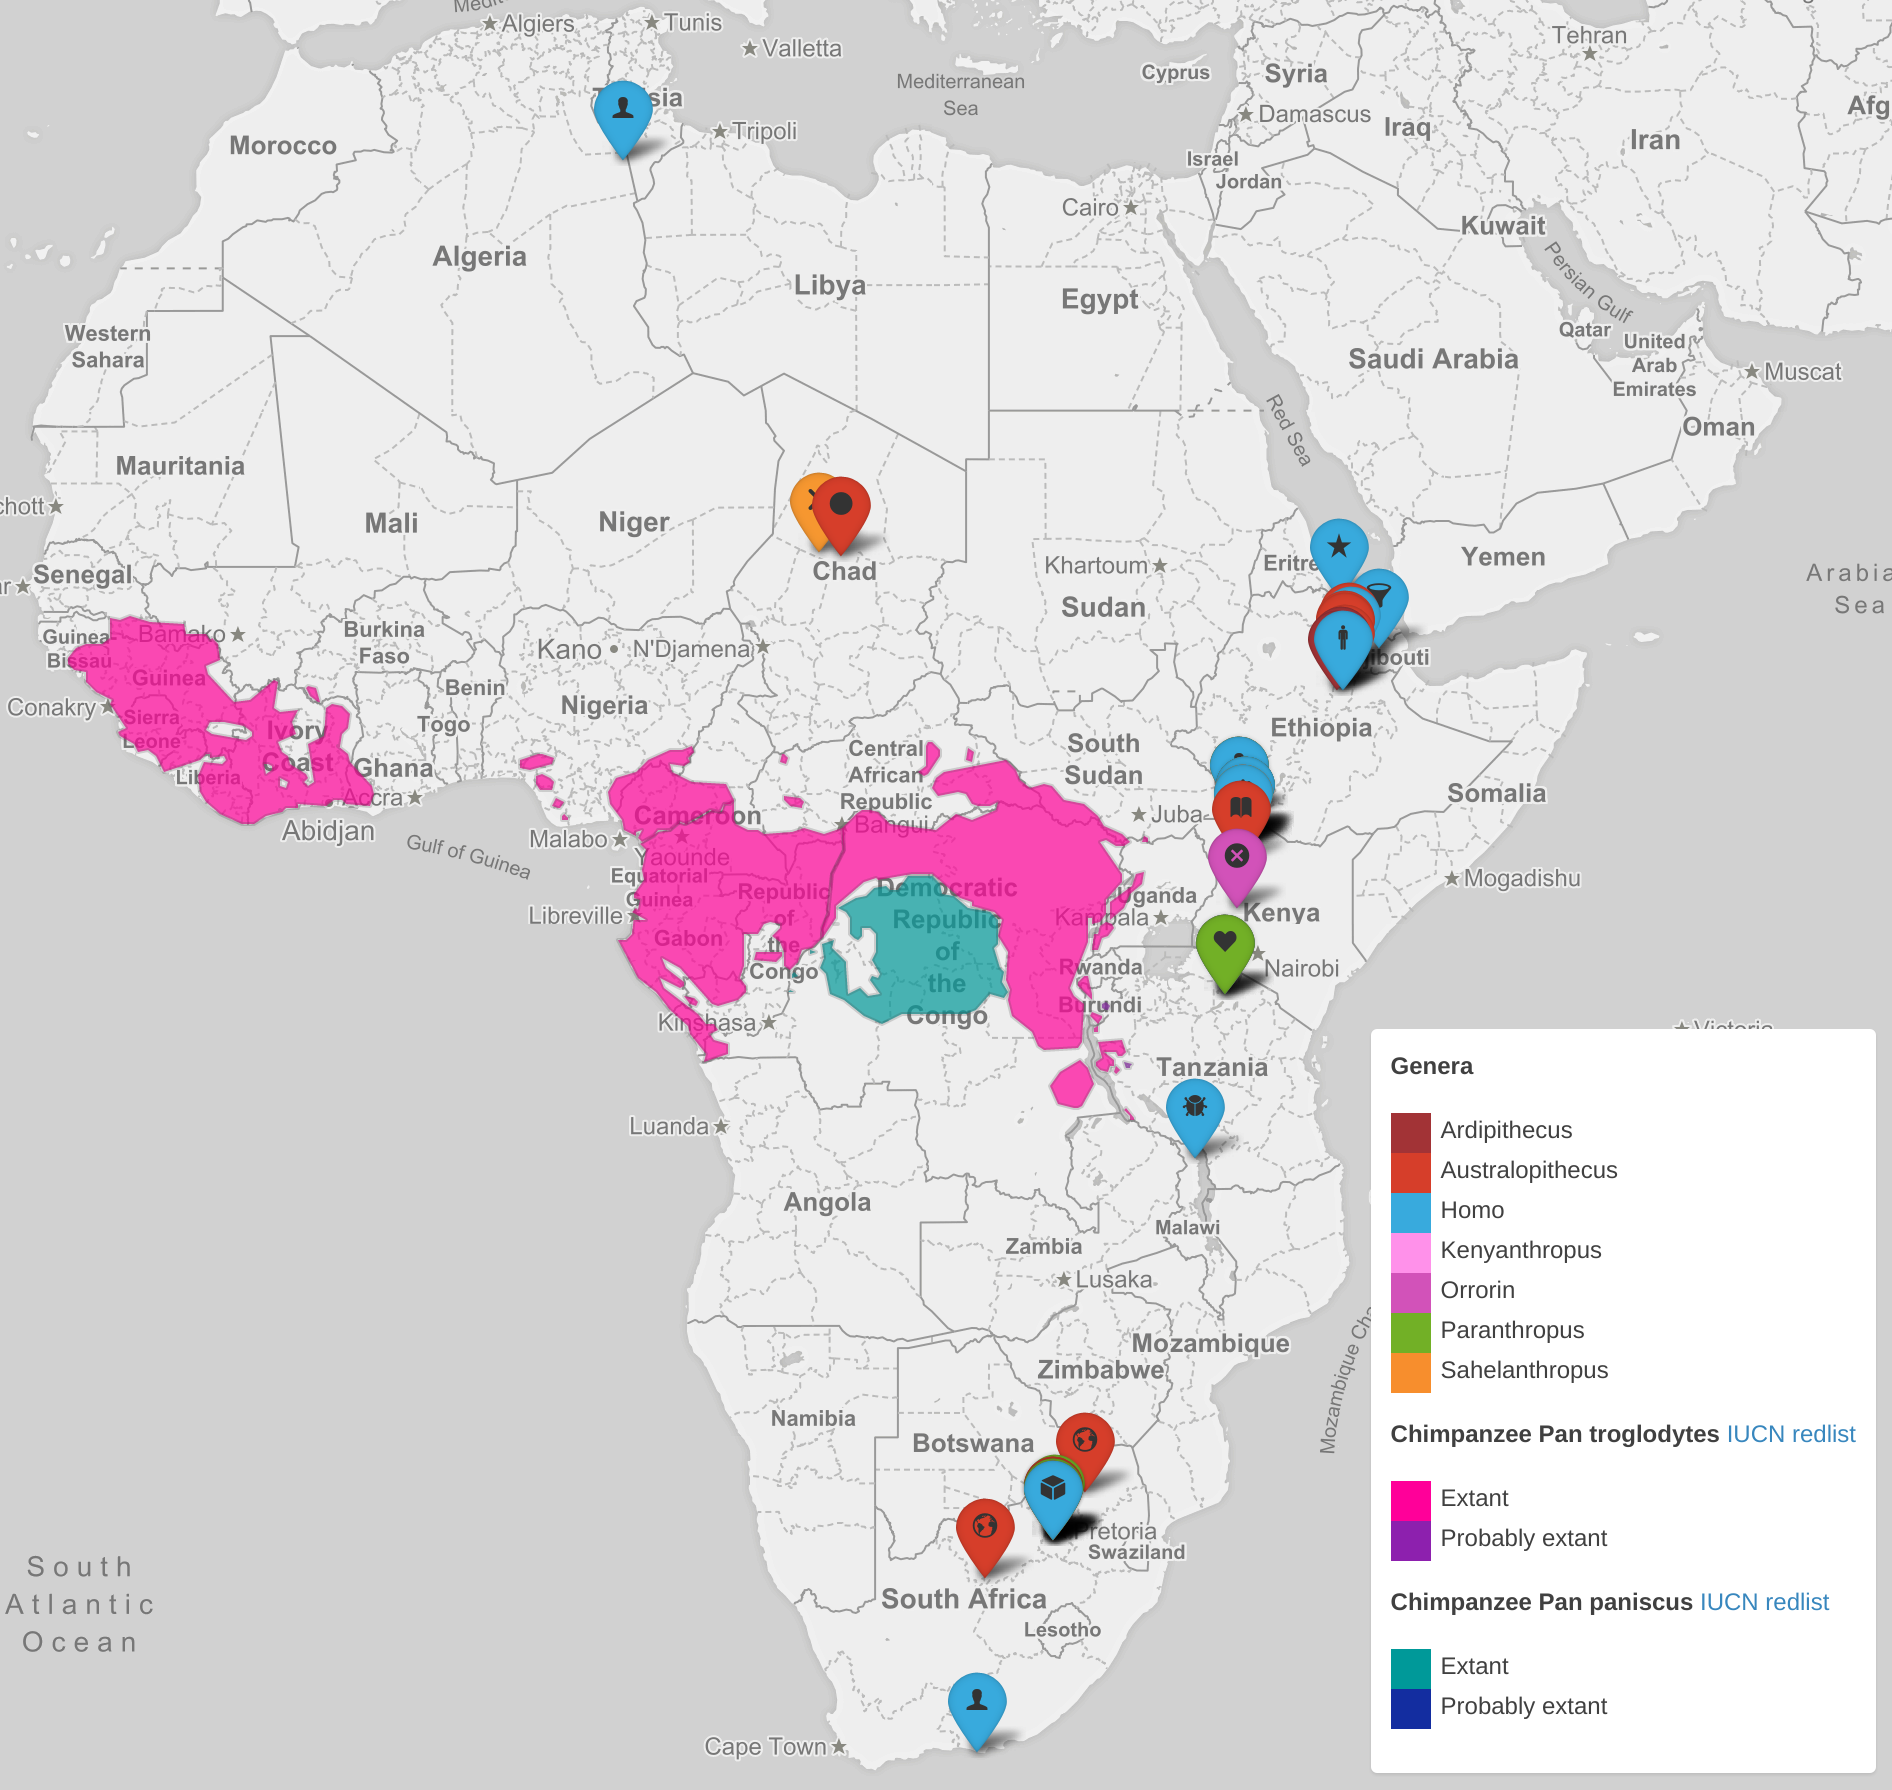
\includegraphics[width=\textwidth]{figs/chimpanzee}
  \caption{Distribution of Chimpanzee [IUCN redlist \url{http://maps.iucnredlist.org/map.html?id=15933}, \url{http://maps.iucnredlist.org/map.html?id=15932}] and fossils}
  \label{fig:chimpanzee}   
\end{figure}     

Fossils from four genera (Ardipithecus, Kenyanthropus, Orrorin and Sahelanthropus) were excluded from the analysis on the basis that there is no fossil evidence that they persisted after 3 MYA. Our range of candidate species can be restricted to those in supplementary Table A.1.

We then used further data on geo-temporal proximity of one species to another to develop mathematical models to quantify the probability of HSV2 infection transmission so as to assess the likelihood that each of these species further transmitted HSV2 to another hominin (see methodology section for further detail of the model). If HSV2 was transmitted to \textit{Homo erectus}, parsimony militates against the need for a further cross-species transmission event to be invoked to explain the infection of modern humans by HSV2. Simple vertical mother-to-child or horizontal (sexual) transmission of the virus through the genus Homo from this point would be sufficient as the ancestor-descendent path from \textit{Homo erectus} to \textit{Homo sapiens} is relatively secure~\cite{Maslin2015}.

\section*{Discussion}
\subsection*{Transmission of HSV2}
Our analysis suggests that \textit{Homo rudolfensis} was the most likely intermediate host of HSV2 between chimpanzees and the ancestors of \textit{Homo sapiens}. The combined inference analysis of a Bayesian Network, considering the presence of HSV2 in both ancestral-chimpanzees and \textit{Homo erectus}, revealed \textit{A~afarensis} (90.33\%), \textit{H~habilis} (60.85\%), \textit{P~boisei} (57.3\%), and \textit{H~rudolfensis} (42.6\%) to be the likely intermediary hosts. However, \textit{A~afarensis} could only transmit to \textit{A~africanus}, which had a mere 6\% chance of being infected by HSV2. This narrowed the possibility of transmission through \textit{H~habilis}, \textit{P~boisei} and \textit{H~rudolfensis}, either directly or as intermediary hosts. Infection Prevalence (HSV2-IP) describes the probability of HSV2 infection based on the proximity to the rain forest habitat and the duration (difference between the first and the last appearance datum) using a beta distribution. While, the Infection Transmission (HSV2-IT) model assigns probability values (edge costs) to the DAG utilising the temporal overlap between hominin species and their geographic proximity to one another. The A* algorithm estimated the minimum path costs of 0.252 and 0.87 for the transmission route through \textit{Homo rudolfensis} for both HSV2-IP and HSV2-IT based DAGs, respectively. Bayesian network inference analysis estimated the highest probability of HSV2 transmission (11.6\%) to the ancestors of \textit{Homo sapiens} through \textit{rudolfensis}. Transmission through \textit{boisei} and \textit{habilis} was estimated to be 9.3\% and 7.8\% probable. A* optimal path traversals also predicted \textit{boisei} and \textit{habilis} to be the second (~5\% less likely than \textit{rudolfensis}) and the third (~7\% less likely than \textit{rudolfensis}) most probable routes. These algorithms predict a single intermediate hominin to be more likely than multiple-levels of transmissions. The A* algorithm and the Bayesian network inference have clearly demonstrated that \textit{Homo rudolfensis} is the most likely intermediate hominin host.  

Tropical refugia during hot dry periods may have driven chimpanzees into higher concentrations in certain areas, driving them into contact and competition with \textit{Homo rudolfensis}. Violent confrontation or predation in combination with hunting and butchery practices would have provided a viable route of transmission for HSV2.  While no stone tools have to date been found in the same archaeological strata as \textit{Homo rudolfensis} fossils it is a logical  assumption that they would have been extensively used by this species~\cite{Ungar2006,DelaTorre2003} as Oldowan or Mode 1 stones tools are widely distributed in the same spatial-temporal localities as \textit{Homo rudolfensis} fossils~\cite{stern1993structure,Leakey2012}. \textit{Paranthropus aethiopicus}, \textit{P.~boisei}, and \textit{P.~robustus} are associated with the Olduwan stone tool complex~\cite{DeHeinzelin1999}, and \textit{P~boisei} explicitly with butchery~\cite{Dominguez-Rodrigo2013} lending support to the hypothesis that bushmeat hunting and butchery may have led to the initial transmission of HSV2 to the hominins. \textit{A~afarensis}, although a tool user, can be excluded both on statistical grounds and by the lack of evidence for hunting and butchery within this species which instead used tools to scavenge the carcasses left behind by savannah predators~\cite{Dominguez-Rodrigo2010,Domalain2016}.

Although ChHV1 causes outbreaks of oral and pharyngeal lesions in chimpanzees in a manner similar to HSV1, in hominins contracting the virus which was to become HSV2, the oral niche was already occupied by HSV1. This may have protected the hominin first infected with HSV2: pre-existing infection with HSV1 reduces the likelihood that subsequent infection with HSV2 will be symptomatic~\cite{Langenberg1999}, and also reduces the risk of HSV2 meningitis~\cite{Aurelius2012}. HSV2 may have been forced to adapt to a different mucosal niche in order to reduce competition from the co-evolved, native HSV1.

We suggest that the mode of transmission of HSV2 into hominins was most likely through hunting injuries (eg chimpanzee bites or cuts sustained during meat processing), although onwards transmission into the ancestors of \textit{Homo sapiens} could have been sexual (horizontal) or a result of hunting injuries (vertical). There are many reports of transmission of B virus (\textit{Cercopithecine herpesvirus 1}), the cercopith homolog of HSV1 and ChHV1, to humans, where disease ranges from mild to fatal. Transmission has occurred from bites and scratches, needle sticks and even scratches from cage bars that are contaminated with B virus-positive bodily fluids~\cite{Huff2003}. Onwards transmission between humans has been reported to occur~\cite{CentersforDiseaseControlCDC1987}. Human herpesvirus 1 can infect other primates, from gorillas~\cite{Gilardi2014} to owl monkeys~\cite{Melendez1969}, typically causing fatal disease in species more distantly related to Homo sapiens, while causing oral lesions and milder disease in great apes such as Gorilla \textit{beringei graueri}~\cite{Gilardi2014}. We therefore infer that herpes simplex-like viruses spread relatively easily between individuals even across species barriers, increasing the chances of transmission between hominins and other primates from close contact such as hunting, butchery, inter-personal violence or sexual contact. Evidence for close hominin-hominid contact is also found in other `heirloom' human pathogens~\cite{Houldcroft2017a}.

The high prevalence of HSV2 in central and eastern Africa (see Figure A.1) and interactive maps at \url{https://wadhamite.github.io/hsv-mapping}) is consistent with the limited genetic data available from African HSV2 isolates. A study from Burrel and colleagues~\cite{Burrel2015} showed that HSV2 can be divided into African and worldwide lineages on the basis of diversity in gene UL30. Furthermore, they found evidence of gene flow from HSV1 into HSV2, and speculate that the flow of HSV1 loci into the worldwide HSV2 lineage may have helped this lineage of HSV2 to further adapt to human hosts, and so spread more successfully around the world from around 41kya~\cite{Burrel}. Two recent studies have significantly increased the number of whole HSV2 genomes available for analysis, contributing to our knowledge of HSV2 diversity~\cite{Szpara2014,Kolb2015}, however precise geographic origins of each sample are not available. More whole HSV2 genomes from central and east Africa, with clear country of origin data, are needed to enrich this picture, as our model predicts that individuals from east Africa are also likely to carry ancient HSV2 lineages. 

The time-depth of ancient DNA analysis is dually limited by technology and preservation of DNA. Similarly the archaeological and fossil records suffer from differential rates of preservation and gaps that can never be filled because the material has simply not survived.  Our analysis has allowed the reconstruction of hominin/human-disease interaction well beyond the horizon of ancient DNA and at a level that is invisible to the fossil and archaeological records. Demonstrating the potential for using modern disease genetics to better understand the evolutionary interaction between humans and disease in deep time.

\section*{Methods}
\subsection*{HSV2 prevalence data, hominin fossil data and chimpanzee and tropical rainforest geographic range data}

We collated African hominin spatial-temporal data on hominin fossil species extant between 100 KYA and 3 MYA. Spatially, latitude and longitude of site location was used to provide a data point for each species. Temporally, dating was used to provide a first appearance datum (FAD) and last appearance datum (LAD) for each species (supplementary data). GIS data on the range of \textit{Pan troglodytes} and \textit{Pan paniscus} was provided by the IUCN Red List~\cite{Oates2008}. Tropical rainforest distribution between 1.4 and 3 MYA was acquired from the K\"{o}ppen-Geiger climate classification dataset~\cite{Peel2007}. This was treated as a proxy for the ancient range of chimpanzees. Data on the prevalence of herpes simplex virus 2 between 2000 and 2015 was taken from the supplementary materials of Looker~\cite{Looker2015}, with additional country data (see supplementary material). 

\subsection*{Network analysis}

To establish the most probable transmission route of HSV2 from chimpanzees to modern humans, it is important to identify potential species that may have been intermediary hosts. At first, hominins present within the 1.4 - 3 MYA confidence window of chimp-hominin transmission were identified. Their distance to tropical rainforest was calculated: only species with fossil remains found within 400 km of tropical rainforest were considered as putative species for initial ancestral-chimp-hominin HSV2 transmission. A matrix of spatio-temporal distances was then calculated to map distances between nearest neighbours of each species and also to calculate their temporal overlap within the fossil record. Network analysis was peformed using AI space graph search and decision network tools~\cite{poole2010artificial}.

\subsubsection*{Optimal path traversal}
A network of possible transmission routes of HSV2 from ancestral-chimpanzees to humans through different potential hominims was developed as a Directed Cyclic Graph (DAG) $G = (V, E)$ comprising of a set of nodes ($V$), representing potential intermediary hosts, and edges ($E$) connecting the nodes, which represents the direction of transmission between species. Infection Prevalence (HSV2-IP) and Infection Transmission (HSV2-IT) models assign probability value (edge costs) to the DAG utilising the temporal overlap between hominin species and their geographic proximity to rainforest habitat and one another. More details about the probability models are discussed in the next section. A Conditional Probability Table (CPT) is calculated to determine the nodal heuristics. Ancestral-chimpanzees and \textit{Homo erectus} formed the start node and the target node of the DAG. 

The A* pathfinding algorithm~\cite{Hart1968} was used on the DAG to identify the most probable transmission (optimal path) route for HSV2. The A* algorithm is the most widely used path-finding algorithm. A* is an informed search algorithm that searches through all possible paths to the target that yields the smallest cost. This is done by combining information on favouring vertices that are close to the starting point and information on favouring vertices that are close to the goal. At each time-step A* algorithm selects the path at a given vertex $n$ that has the lowest $f(n) = g(n) + h(n)$. Where $g(n)$ represents the exact cost of the path from the starting point to any vertex $n$, and $h(n)$ represents the heuristic estimated cost from vertex $n$ to the goal. A* balances the two as it moves from the starting point to the goal. The A* algorithm evaluates the most probable transmission route, by minimising the traversal costs based on the edge cost and nodal heuristics of the transmission network graph.

\subsubsection*{Bayesian inference}
A Bayesian network or a belief network is a graphical structure that allows us to represent and reason about an uncertain domain. The nodes are variables, and edges represent direct links between nodes. The process of conditioning (also called probability propagation or inference) is performed via a ``flow of decisions'' through the network, which involves computing the posterior probability distribution for a set of query nodes, given values for some evidence (or observation) nodes. An important consideration in all Bayesian-based methods is the choice of a prior. An empirical Bayesian method that estimates the likelihood of HSV2 infection using a prior beta distribution, which is an approximation to a hierarchical Bayesian approach is adopted~\cite{Murphy2012,Farine2015}. Bayesian networks provide full representations of probability distributions over their variables, which allows to infer upon any subset of variables. A Conditional Probability Table (CPT) is generated for all possible combinations of a dichotomous outcome for each variable (HSV2 infection is true or false). The ``Combined Inference'' approach is adopted to evaluate the probable intermediary hosts, by conditioning the ancestral-chimpanzee and \textit{Homo erectus} nodes for the presence of HSV2. A ``Diagnostic reasoning''~\cite{Korb2003} was carried out to evaluate the most probable intermediate hosts for the transmission of HSV2 from ancestral-chimpanzees to \textit{Homo sapiens}. 

\subsubsection*{HSV2-Infection Prevelance (HSV2-IP) model}
This model describes the probability of HSV2 infection based on the proximity to the rain forest habitat and the duration (difference between the first and the last appearance datum)  using a beta distribution. The probability density function is defined as:

\begin{equation}
PDF: \frac{x^{\alpha - 1}(1 - x)^{\beta - 1}}{B(\alpha, \beta)} \qquad \mathrm{where} \qquad B(\alpha, \beta) = \frac{\Gamma(\alpha)\Gamma(\beta)}{\Gamma(\alpha + \beta)}
\end{equation}

Where, $\Gamma$ defines a gamma distribution function, $\alpha$ is the time period of existence of the species in 100,000 years and $\beta$ is the spatial distance of the fossil from the rainforest in kilometres. Monte-carlo simulations were performed to sample from the distributions to populate the edge costs. A minimum overlap threshold of 10\% is considered for possible transmission of HSV2 from one species to another. 

\subsubsection*{Stochastic modelling of infection transmission}
The Susceptible - Infection - Recovered (SIR)~\cite{callahanspread} is one of the most widely used model in epidemiological system. In the stochastic version of the SIR model, the continuous variables are replaced by discrete numbers, and the process rates are replaced by process probabilities. At time `t` the probability of a new susceptible host is infected is modelled as an exponential distribution, which is epidemiologically incorrect for most diseases~\cite{Wearing2005,Bailey1975,sartwell1950distribution}, i.e., the rate of leaving the exposed is independent of the time spent on the host. Wearing et al~\cite{Wearing2005} suggested a more realistic distribution of latent and infectious periods, with a stronger central tendency:

\begin{table*}
	\centering
	\renewcommand{\arraystretch}{1.5}
	\begin{tabulary}{\linewidth}{LCCCC}
		\# of infectives at time ($t$) & =  & 
		Initial number of infectives who are still infectious at time ($t$) & + & 
 Those who have acquired the infection in the time interval $[0, t]$ and are still infectious at time ($t$)			\\ 
\end{tabulary}
\end{table*}

More realistic distributions can be obtained by choosing  probability density function of the infectious period,  p(t) to be a gamma probability density function\cite{Blythe1988,Lloyd2001}.

\subsubsection*{Infection Transmission (HSV2-IT) model}
This model utilising the temporal overlap between hominin species and their geographic proximity to one another to determine the probability of transmission using a gamma distribution. The probability density function of a gamma distribution is given as:

\begin{equation}
PDF:\frac{\beta^\alpha}{\Gamma(\alpha)}x^{\alpha - 1} \exp^{-\beta x}
\end{equation}
in terms of shape $\alpha$ and rate $\beta$. The parameters shape is defined as the ratio of the time period in 1000 years / distance in kilometers and  rate  is defined as the normalised time period $Y / x$, where $x$ is the time period of the species in 1000 years and $Y$ is the time period of anc-chimpanzees. Monte-carlo simulations were performed to evaluate the combined probability of transmission between species is evaluated as mutually exclusive events based on the probability distributions. 

\section*{Data presentation}
The distribution maps were created with custom JavaScripts codes using Leaflet.js library [\url{http://leafletjs.com/}] and interactive maps can be found at \url{https://wadhamite.github.io/hsv-mapping}

\section*{Author contributions}
SJU and CH conceived the study and contributed data. SJU, KK and CH performed the analyses. SJU, KK and CH wrote the paper. All authors approved the publication of the manuscript.

\section*{Acknowledgements}
SJU was funded by Oxford Brookes University. KK and CH were funded by the University of Cambridge. KK is a college research associate at King’s College, Cambridge. The authors would like to thank C Ruis (University College London) for helpful discussion. 

\printbibliography

\clearpage
\section*{Supplementary material}
\renewcommand\thefigure{A.\arabic{figure}}    
\setcounter{figure}{0} 
\renewcommand\thetable{A.\arabic{figure}}    
\setcounter{table}{0} 

\begin{figure}[!h]
	\centering
	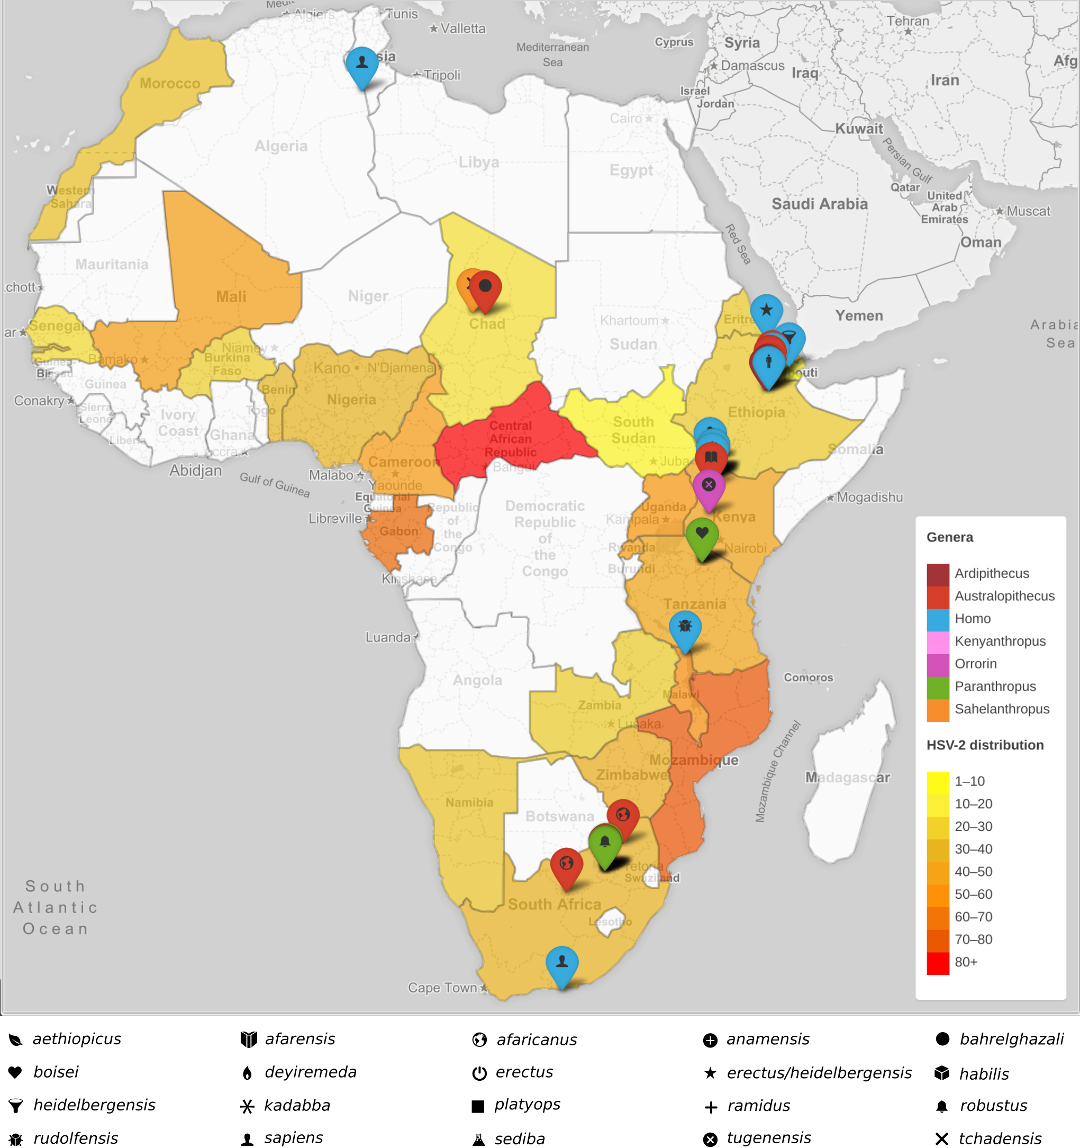
\includegraphics[width=\textwidth]{figs/fossils}
	\caption{Prevalence of HSV2 in Africa}
	\label{fig:hsv2}   
\end{figure}  

\clearpage
\centering
\textbf{Table A.1.} Fossil hominins with the potential to acquire - HSV2 from ancestral chimpanzee\\
\renewcommand{\arraystretch}{2}
\tymin=50pt
\tymax=200pt
\begin{ltabulary}{L|CCCL}
	
	\toprule
	\textbf{Species} &  \textbf{Type specimen} & 	\textbf{Locations (type specimen)} &  \textbf{Age (000s BP)} & \textbf{Publication (suggesting a new species)}\\ 
	\midrule
	\endfirsthead
	
	\midrule
	\textbf{Species} &  \textbf{Type specimen} & 	\textbf{Locations (type specimen)} &  \textbf{Age (000s BP)} & \textbf{Publication (suggesting a new species)}\\ 
	\midrule
	\endhead
		 
	% Footer to say continued on next page
	\midrule
	\multicolumn{5}{r}{Continued on next page}\\
	\midrule
	\endfoot
	
	% Footer on the last page of the table
	\bottomrule
	\endlastfoot
	

	\textit{Australopithecus afarensis} & LH4 (mandible) &
	East Africa (Laetoli, Tanzania) & 3900 - 2800 & 
	Johanson DC, White TD and Coppens Y 1978 A new species of the genus Australopithecus (Primates: Hominidae) from the Pliocene of eastern Africa. \textit{Kirtlandia 28: 2-14.}\\
	
	
	\textit{Australopithecus africanus} & Taung 1 (cranium) &
	Southern Africa (Taung, SA) & 2800 - 2300 &
	Dart RA 1925 Australopithecus africanus: The man-ape of South Africa. \textit{Nature 115: 195-199.}\\
	
	
	\textit{Australopithecus gahri} & BOU-VP-12/130 (cranium) &
	East Africa (Bouri, Ethiopia) & 2500 &
	Asfaw B, White T, Lovejoy O, Latimer B,. Simpson S and Suwa G 1999 Australopithecus garhi: A new species of early hominid from Ethiopia. \textit{Science 284: 629-635.}\\
		
	

	\textit{Paranthropus aethiopicus} & Omo 18-1967-18 (mandible) &
	East Africa (Omo, Kenya) & 2700 - 2300 &
	Arambourg C and Coppens Y 1967 Sur la d\'{e}couverte, dans le Pl\'{e}istoc\`{e}ne inf\'{e}rieur de la vall\'{e}e de l’Omo (Éthiopie), d’une mandibule d’australopith\'{e}cien. \textit{Comptes Rendus de l’Acad\'{e}mie des Sciences, Paris, series D, 265: 589-590.}\\
	
	
	\textit{Paranthropus robustus} (including \textit{Paranthropus crassidens}, SK 48) &
	TM 1517 (various) &	Southern Africa (Kromdraai, SA) &	1800 - 1000 &
	Broom R 1938 The Pleistocene anthropoid apes of South Africa. \textit{Nature 142: 377-379.}\\
	
	
	\textit{Paranthropus boisei} & OH 5 (cranium) & 
	East Africa (Olduvai Gorge, Tanzania) & 1750 - 1200 &
	Leakey LSB 1959 A new fossil skull from Olduvai. \textit{Nature 184: 491-493.}\\
	
	
	\textit{Homo habilis} (Australopithecus?) & OH 7 (mandible) & 
	East Africa (Olduvai Gorge, Tanzania) & 2500 - 1600 & 
	Leakey LSB, Tobias PV and Napier JR 1964 A new species of the genus Homo from Olduvai Gorge, Tanzania. \textit{Nature 202: 308-312.}\\
	
	
	\textit{Homo rudolfensis} (Kenyanthropus?) & KNM-ER 1470 (cranium) & 
	East Africa (Koobi Fora, Kenya) & 2400 - 1800 &
	Leakey RE 1973 Evidence for an advanced Plio-Pleistocene hominid from east Rudolf, Kenya. \textit{Nature 242: 447-450.} \\
	
	
	\textit{Homo erectus} & KNM-ER 992 (mandible) & 
	Africa (Koobi Fora, Kenya) & 2000 - 600 & 
	Groves CP and Mazák V 1975 An approach to the taxonomy of the Hominidae: Gracile Villafranchian hominids of Africa. \textit{Casopis pro Mineralogii Geologii 20: 225-247.} \\

\end{ltabulary}

\end{document}